\documentclass[12pt]{article}
\usepackage{amsmath}
\usepackage{amssymb}
\usepackage{graphicx}
\usepackage{float}
\usepackage[margin=2cm]{geometry}
\usepackage[parfill]{parskip}
\usepackage{listings}
\usepackage{xcolor}
\usepackage[style=numeric-comp,useprefix,hyperref,backend=bibtex]{biblatex}
\definecolor{dark-green}{RGB}{0,175,0}
\definecolor{dark-red}{RGB}{200,0,0}
\graphicspath{ {./pictures/} }
\addbibresource{report.bib}
\DeclareUnicodeCharacter{202F}{\,}
\begin{document}
	\title{NAML Project Report - Group 14\\\vspace{20pt}
		\Large{Music Genre Classification using}\\
		\large{k-Nearest Neighbours\\ Nearest Centroid\\ Multiclass SVM}\\
		\date{February 2022}
		\large{-\\}
		\large{by Silvia Marino (codice persona) and Francesco Panebianco (10632465)\\}
		\small{DEIB - Politecnico di Milano}
	}
	\maketitle
	\tableofcontents
	\newpage
	\section{Introduction}
	\paragraph{Scope}\mbox{}\\\newline
	The scope of this project is to create a music genre classifier using the machine learning algorithms \textit{k-Nearest Neighbours} and \textit{Multiclass SVM}, which were assigned to our group. The project is part of the evaluation of the “Numerical Analysis for Machine Learning” course, which is part of the first semester of the first year of Master’s Degree in Computer Science and Engineering at Politecnico di Milano. Given the similarities between \textit{k-Nearest Neighbours} and \textit{Nearest Centroid}, we chose to implement the latter as well, comparing its performance to the former, even though it is outside the specification of the project.\\ 
	
	\paragraph{The Dataset}\mbox{}\\\newline
	The dataset assigned to our project is the notorious \textit{GTZAN Genre Collection}\cite{marsyas}, which contains 100 different extracts from 10 different music genres, provided in .wav (Waveform Audio File Format). The genres considered are: 
	
	\begin{itemize}
		\item Blues 
		\item Classical 
		\item Country 
		\item Disco 
		\item Hip Hop 	
		\item Jazz 
		\item Metal 
		\item Pop 
		\item Reggae 
		\item Rock 
	\end{itemize}

	As it can be seen, genres that share similarities are included in the dataset (e.g. Blues and Jazz), but also dramatically different types of music such as Rock and Classical, which we expect the algorithms to classify with higher precision.
	
	The \textit{.wav} file format used by the dataset is the most common uncompressed audio file format in Microsoft Windows systems for. It was developed by IBM and Microsoft, for storing an audio bitstream on PCs\cite{wave}.\\
	
	\begin{figure}[H]
		\hspace{100pt}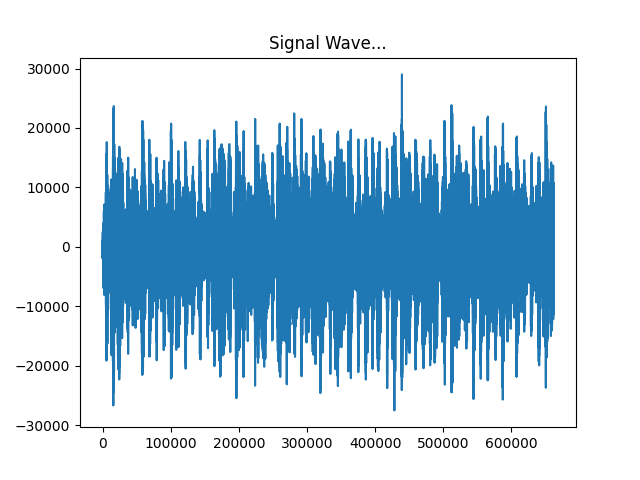
\includegraphics[scale=0.7]{waveform}
		\caption{Plotted waveform of blues.00000.wav}
	\end{figure}
	
	
	This kind of files are managed in Python by using the \textit{wave} module, which provides convenient functions to work with the WAV sound format. In our case, the audio samples are provided as 22050Hz Mono 16-bit 30 second tracks\cite{marsyas}, which are easily transformed into a numpy array of \textit{int16}.\\
	The picture above is the result of the following code:
	\begin{lstlisting}[language=Python]
		import wave
		import matplotlib.pyplot as plt
		import numpy as np
		
		test_file = wave.open('genres/blues/blues.00000.wav', 'rb')
		# Extract Raw Audio from Wav File
		signal = test_file.readframes(-1)
		signal = np.frombuffer(signal, dtype='int16')
		test_file.close()
		
		plt.figure(1)
		plt.title("Signal Wave...")
		plt.plot(signal)
		plt.show()
		
	\end{lstlisting}
	\newpage
	
	\paragraph{Feature Extraction}\mbox{}\\\newline
	For what concerns the features required to classify the genres, our first choice was the triplet \textit{Zero Crossing Rate}, \textit{Average Energy} and \textit{Silent Ratio} as defined in one of the provided papers\cite{comparison}. The extracted features were collected and exported in a csv file to avoid having to extract the feature multiple times, as the complete process took approximately 45 minutes on \textit{Google Colab}.\\
	
	\textbf{Zero Crossing Rate}\\
	It indicates the frequency of signal amplitude sign change, which is in some way related to the average signal frequency. In practice, it is a key feature to classify percussive sounds as it's often correlated with the beat. ZCR records how many waves have passed for a certain time, by giving a positive amplitude a positive value (1) and a negative amplitude a negative value (-1). The implemented formula is as follows:
	
	\begin{equation}
		\text{ZCR}=\dfrac{\sum_{n=1}^N{\bigg|\text{sgn}\ x(n)-\text{sgn}\ x(n-1)\bigg|}}{2N}
	\end{equation}
	
	where sgn $x$ is the \textit{sign function}.\\
	
	\textbf{Average Energy}\\
	It indicates the loudness of the audio signal as a whole, being the average of the square amplitude of the audio signal.
	\begin{equation}
		\text{E}_\text{avg}=\dfrac{\sum_{n=0}^{N-1}{x(n)^2}}{N}
	\end{equation}
	In practice, it corresponds to the loudness of the music within the time slice where it is measured. \\
	
	\textbf{Silent Ratio}\\
	It indicates the proportion of the sound piece that is considered to be \textit{silent}. Silence is defined as a period within which the absolute value of amplitude is below a certain threshold. If we indicate
	\begin{equation}
		SR = \dfrac{\sum_{x(n)<\text{thr}} 1}{N}
	\end{equation}
	In our implementation, silence threshold is derived from the average energy as follows...
	\begin{equation}
		\text{thr}=0.8\sqrt{E_\text{avg}}
	\end{equation}
	\mbox{}\\
	
	\section{k-Nearest Neighbours Classifier}
	In this section it will be explained which methodologies have been used to implement the music genre classifier and how the code has been structure to achieve the results exposed at the end of the report 
	\section{Nearest Centroid Classifier}
	\section{Multiclass SVM Classifier}
		
	\printbibliography
\end{document}